\documentclass[letterpaper,12pt]{article}
\usepackage{tabularx} % extra features for tabular environment
\usepackage{amsmath}  % improve math presentation
\usepackage{float}
\usepackage{pdfpages}

\usepackage{graphicx} % takes care of graphic including machinery
\graphicspath{ {./figures/} }
\usepackage[margin=1in,letterpaper]{geometry} % decreases margins
\usepackage{cite} % takes care of citations
\usepackage[final]{hyperref} % adds hyper links inside the generated pdf file
\hypersetup{
	colorlinks=true,       % false: boxed links; true: colored links
	linkcolor=blue,        % color of internal links
	citecolor=blue,        % color of links to bibliography
	filecolor=magenta,     % color of file links
	urlcolor =blue         
}

%
\setcounter{tocdepth}{4} 
\setcounter{secnumdepth}{4}


\begin{document}

\title{Experiment 7 \protect\\Rectifiers, Capacitors and Inductors}
\author{Ahmet Akman 2442366 \protect\\ Assistant : Uğur Berkay Saraç}
\date{\today}
\maketitle
\newpage
\tableofcontents
\newpage
%\begin{abstract}
%abstract
%\end{abstract}

\section{Introduction} 
In this experiment, as students, we are expected to experiment with rectifiers, capacitor and inductor circuits by completing the steps described in the seventh experiment laboratory manual. Throughout these steps, the half  full rectifier circuit structures and ripple voltages are expected to be learned. The output versus input characteristics is observed by connecting the signal generator to the oscilloscope and the circuit.  Also, the measurement techniques for capacitance of capacitors and inductance of inductors are expected to be expressed and experimented. The results of the steps were recorded and plotted for further comments.
\section{Experimental Results}
In this section, the results of Experiment 7 are discussed. 
\subsection{Step 1}
In this step, circuit shown in the Figure 1  is constructed. 
\begin{figure}[H]
	\centering
   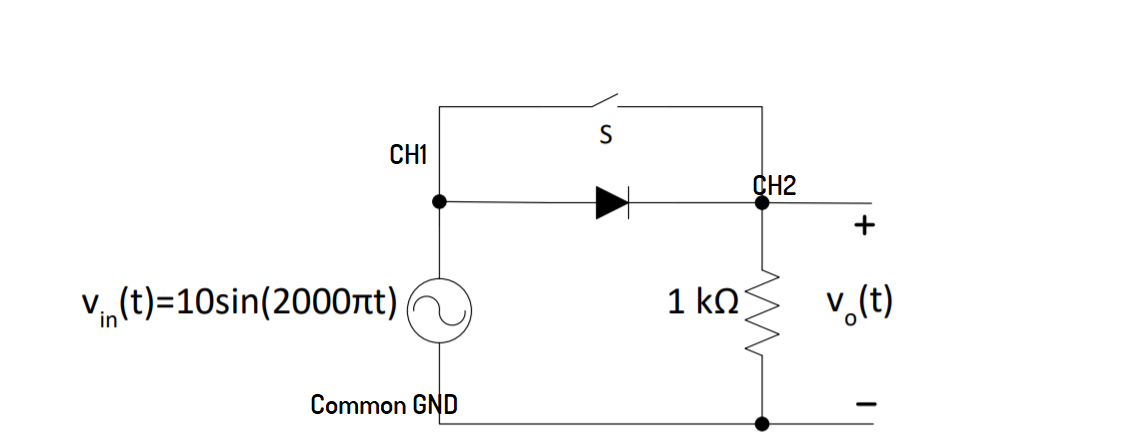
\includegraphics[width=1\textwidth]{half_vave_sch.png}
   \caption{Half wave rectifier circuit}
\end{figure}
\subsubsection{a)}
By connecting the channels of the oscilloscope to the CH1 and CH2 nodes, the plot given in Figure 2 is obtained.
\begin{figure}[H]
	\centering
   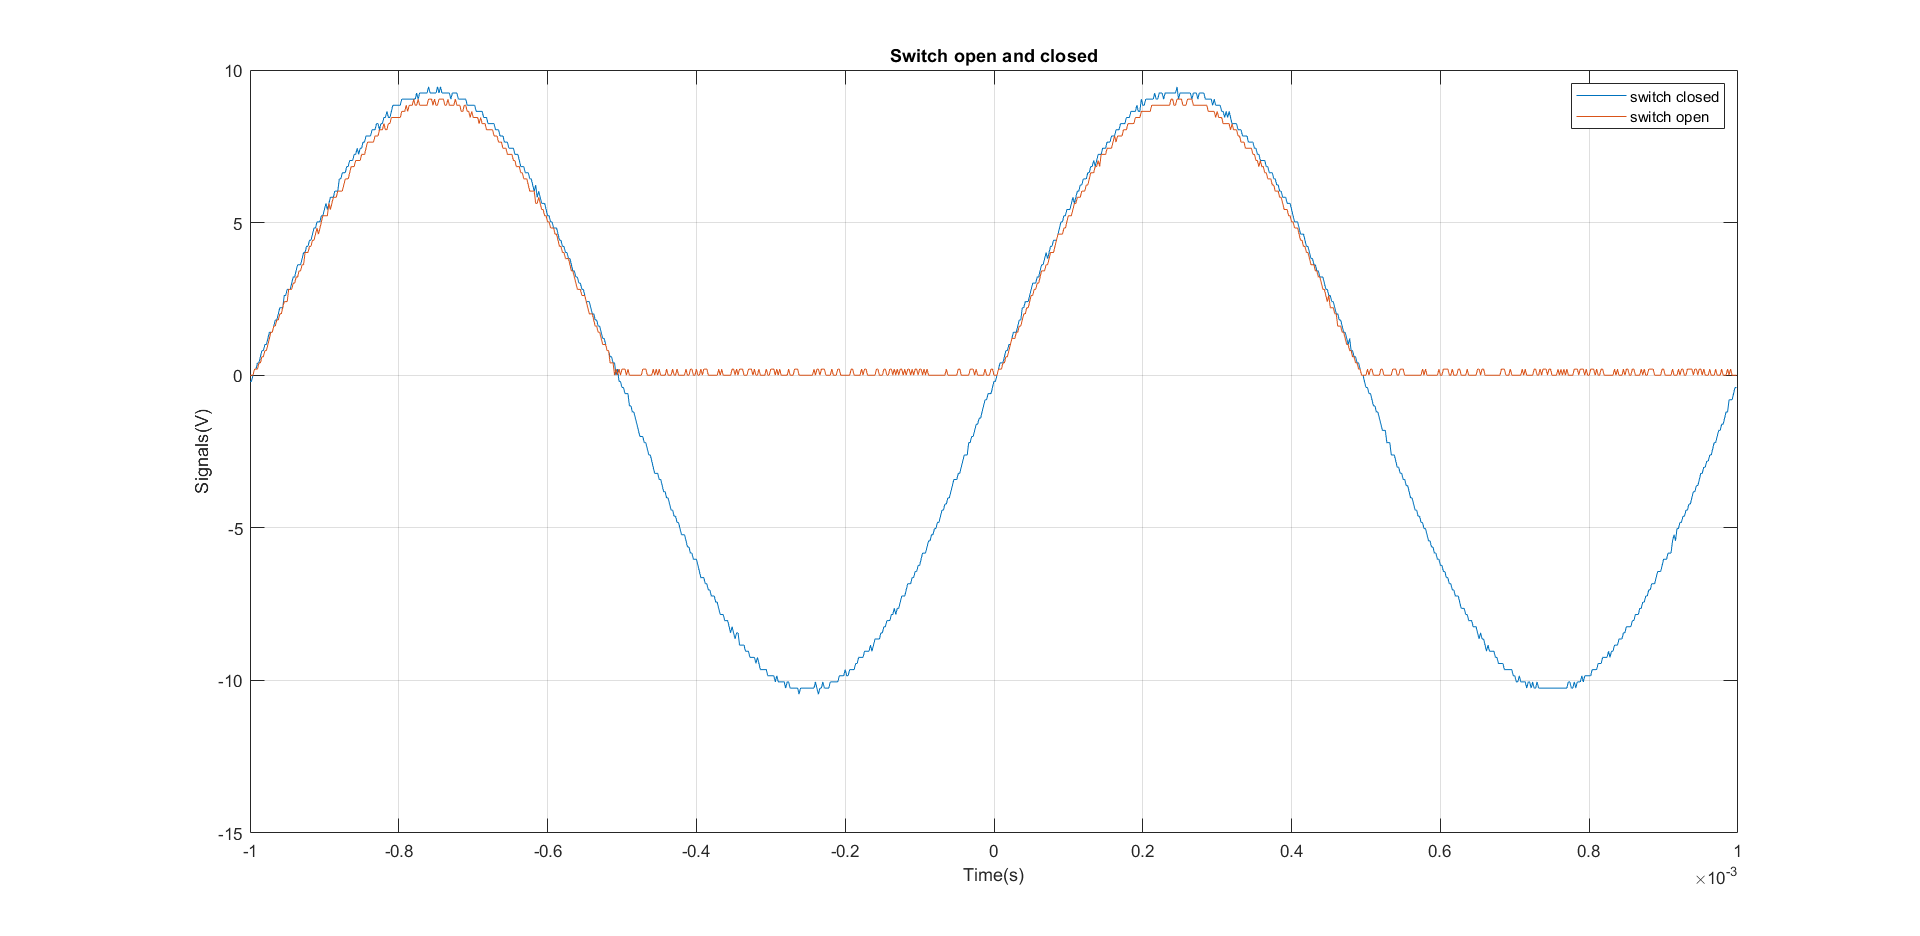
\includegraphics[width=1\textwidth]{1a_plot.png}
   \caption{Output waveforms}
\end{figure}
As a result, it can be said that half wave rectifier is able to allow only positive current to flow.

\subsubsection{b)}
There is a little difference of maximum values of the waveforms. This can be stemmed from the fact that the diode component do not behave ideally and have an opening voltage. This opening voltage should be passed in order diode to allow current pass through. 
\subsection{Step 2}
For this step circuit shown in Figure 3 is set with LEDs. 
\begin{figure}[H]
	\centering
   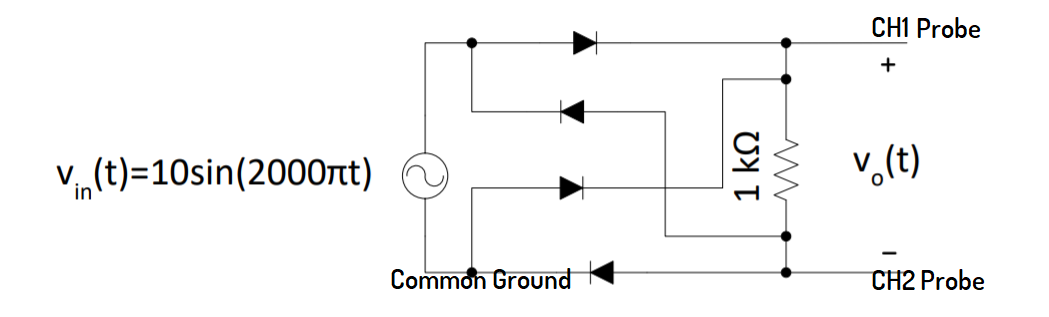
\includegraphics[width=1\textwidth]{full_vave_sch.png}
   \caption{Full wave rectifier circuit}
\end{figure}

\subsubsection{a)}
The plot given in Figure 4 is obtained using the math function of the DSO. 
\begin{figure}[H]
	\centering
   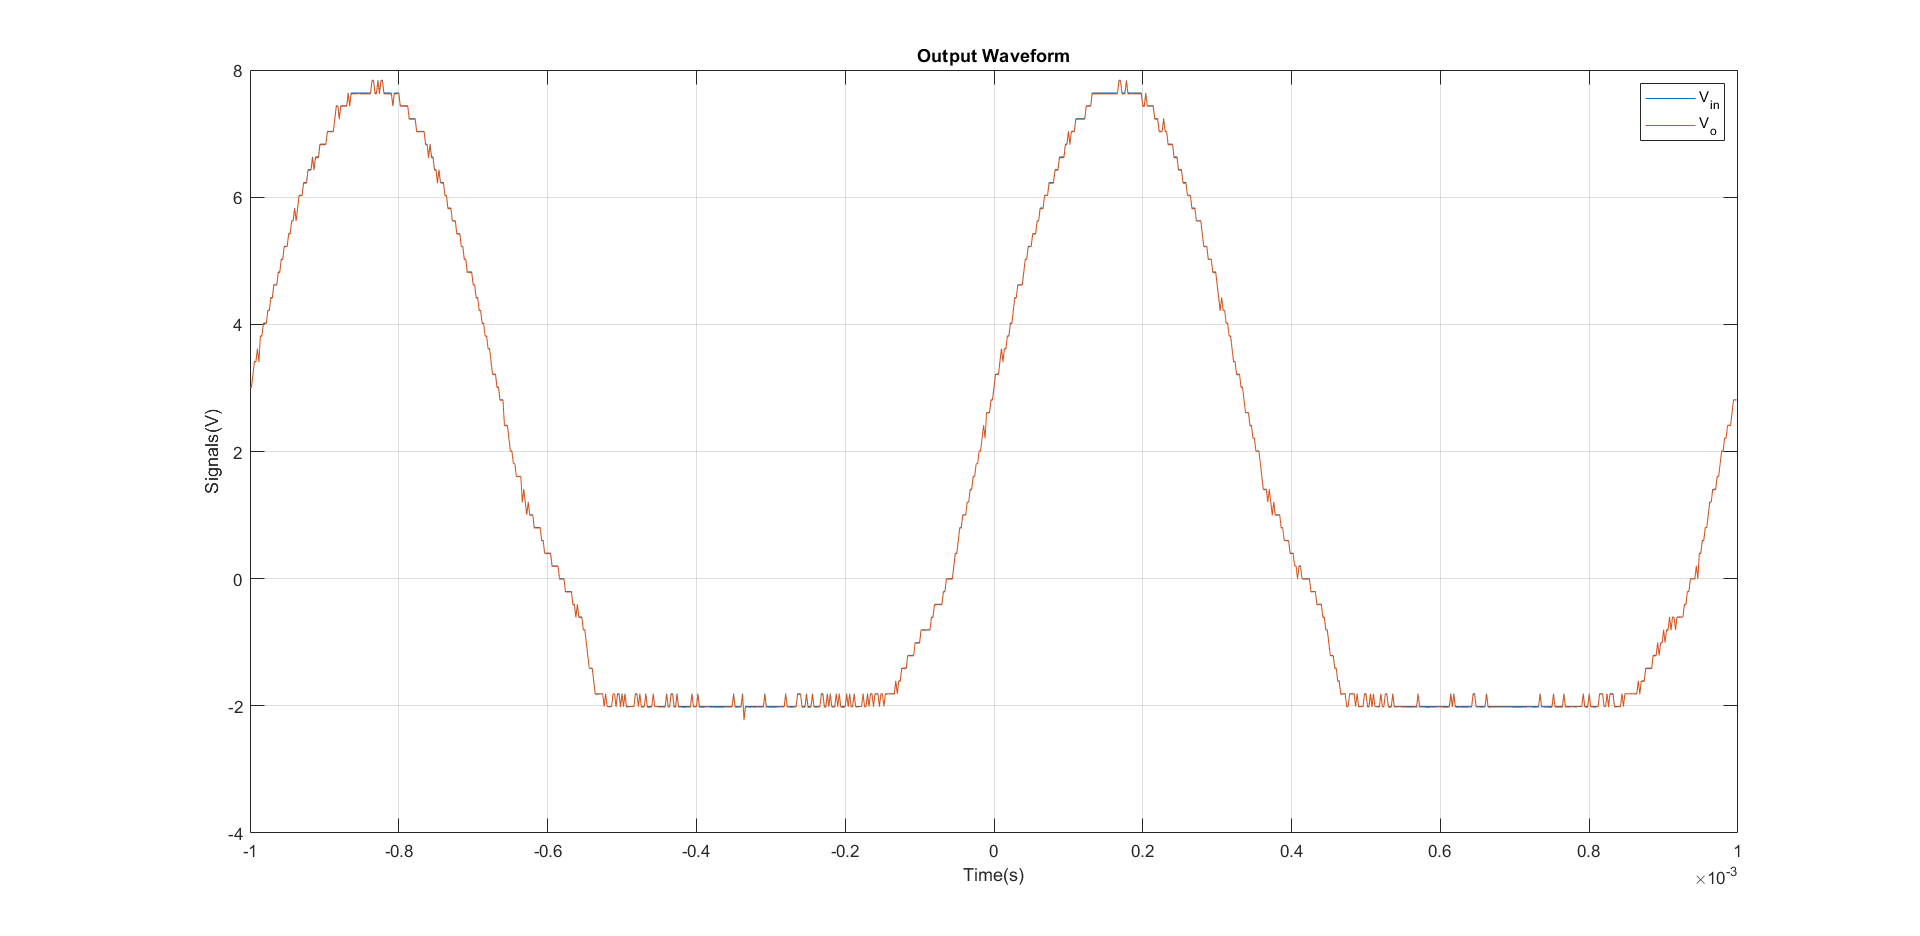
\includegraphics[width=1\textwidth]{2a_plot.png}
   \caption{Output waveforms}
\end{figure}
To solve the grounding problem oscilloscope probes are connected to the nodes expressed in Figure 3. Then the CH2 signal is subtracted from the CH1 signal to get resulting signal. Also even though the input Vp is 10V the resulting signal have the amplitude of 6V. This difference means diodes have 2V opening voltage (2 volts per diode). 

\subsubsection{b)}
The frequency of the signal generator is adjusted to 1Hz. As a result the LEDs have started to blink visibly. Two of the LEDs blinked at the same time, which means when the voltage is positive two of the diodes are active and when the voltage is negative other two of the diodes are active. When the frequency increases , the blink becomes less noticable.
\subsubsection{c)}
The frequency is set to 1kHz and a 0.47\(\mu\)F capacitor is connected parallel to the resistor. The plot given in Figure 5 is obtained.
\begin{figure}[H]
	\centering
   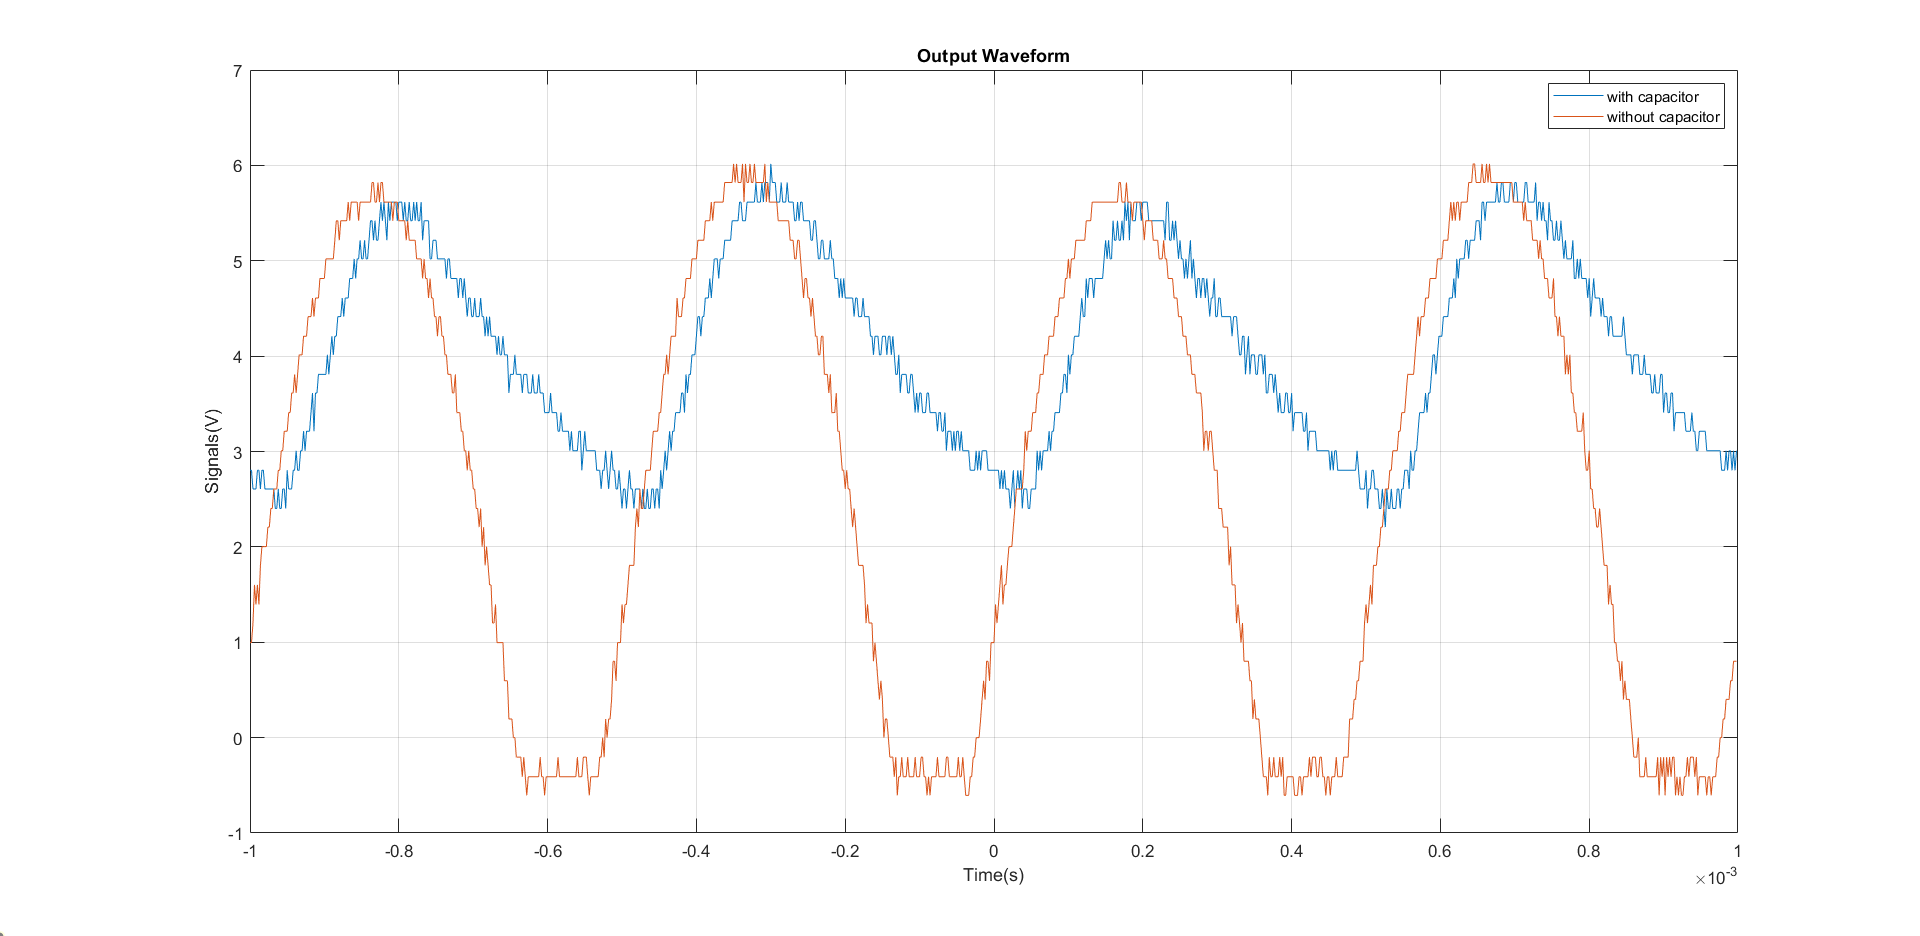
\includegraphics[width=1\textwidth]{2c_plot.png}
   \caption{Output waveforms}
\end{figure}
It can be stated that, when a capacitor is connected the ripple voltage decreases ,and the output look more alike DC. The capacitor discharges when voltage decreasing and helps the node remain its voltage.

\subsection{Step 3}
The circuit given in Figure 6 is built for the Step 3.
\begin{figure}[H]
	\centering
   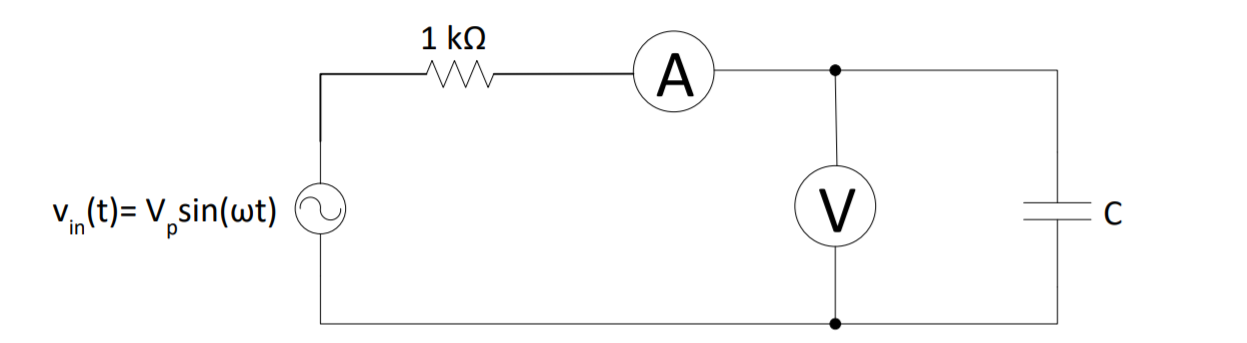
\includegraphics[width=1\textwidth]{PRE3.png}
   \caption{Capacitor measurement circuit}
\end{figure}
Then the RMS voltage measurements are made using digital multimeter. The measurements are given in Table 1.

\begin{table}[H]
	\begin{center}
		\caption{Measurements for the capacitor circuit}
		\vspace{2mm}
		\begin{tabular}{||c | c | c||} 
		 \hline
		   & Capacitor & Resistor \\ [0.5ex] 
		 \hline\hline
		 Voltage Reading & 1.1518 V & 1.69 V  \\ 
		 \hline
		\end{tabular}
\end{center}
\end{table}
By dividing the voltage of the resistor to its resistance value, the current value is obtained as " 0.00169A".
Then using the equation,
\[|z_c| = \frac{1}{\omega C} = \frac{V_{RMS}}{i_{RMS}}\]
so,
\[C = \frac{i_{RMS}}{V_{RMS} \omega}
	\]
The capacitor value is obtained and the LC meter measurement are given in Table 2ç
\begin{table}[H]
	\begin{center}
		\caption{Measurements for the Capacitor}
		\vspace{2mm}
		\begin{tabular}{||c | c | c||} 
		 \hline
		   Datasheet & Calculation & LC meter Measurement \\ [0.5ex] 
		 \hline\hline
		 0.47\(\mu\)F & 0.4670461 \(\mu\)F & 0.48 \(\mu\)F  \\
		 \hline

		\end{tabular}
\end{center}
\end{table}
It can be said that the calculations are consistent with the datasheet and LC meter measurement. The deviation might be stemmed from the negleteced resistances of cables and capacitor. Also, the resistor value might not be exactly 1k\(\Omega\).




\subsection{Step 4}
For Step 4 the circuit given  in Figure 7 is constructed. 
\begin{figure}[H]
	\centering
   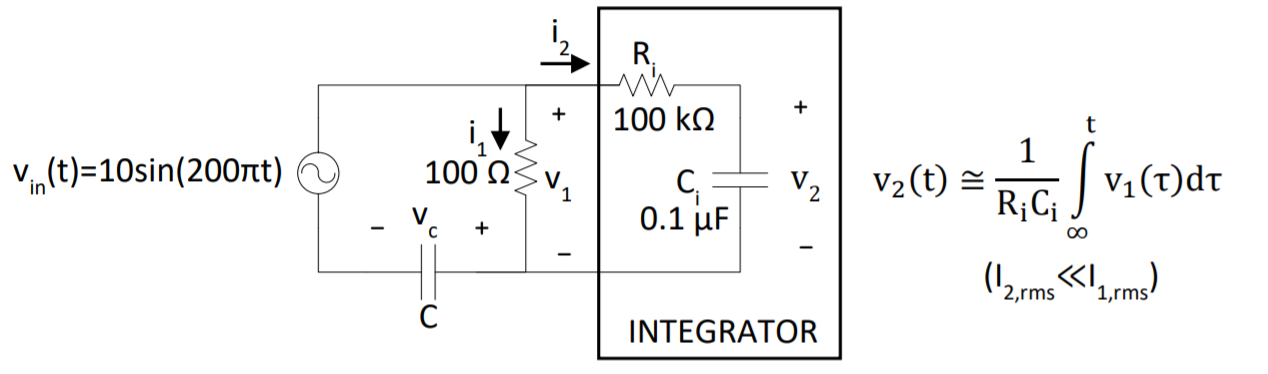
\includegraphics[width=1\textwidth]{PRE4.png}
   \caption{Circuit for the capacitance finding method}
\end{figure}
The circuit is reconstructed in LTSPice simulation environment which is shown in Figure 8.
\begin{figure}[H]
	\centering
   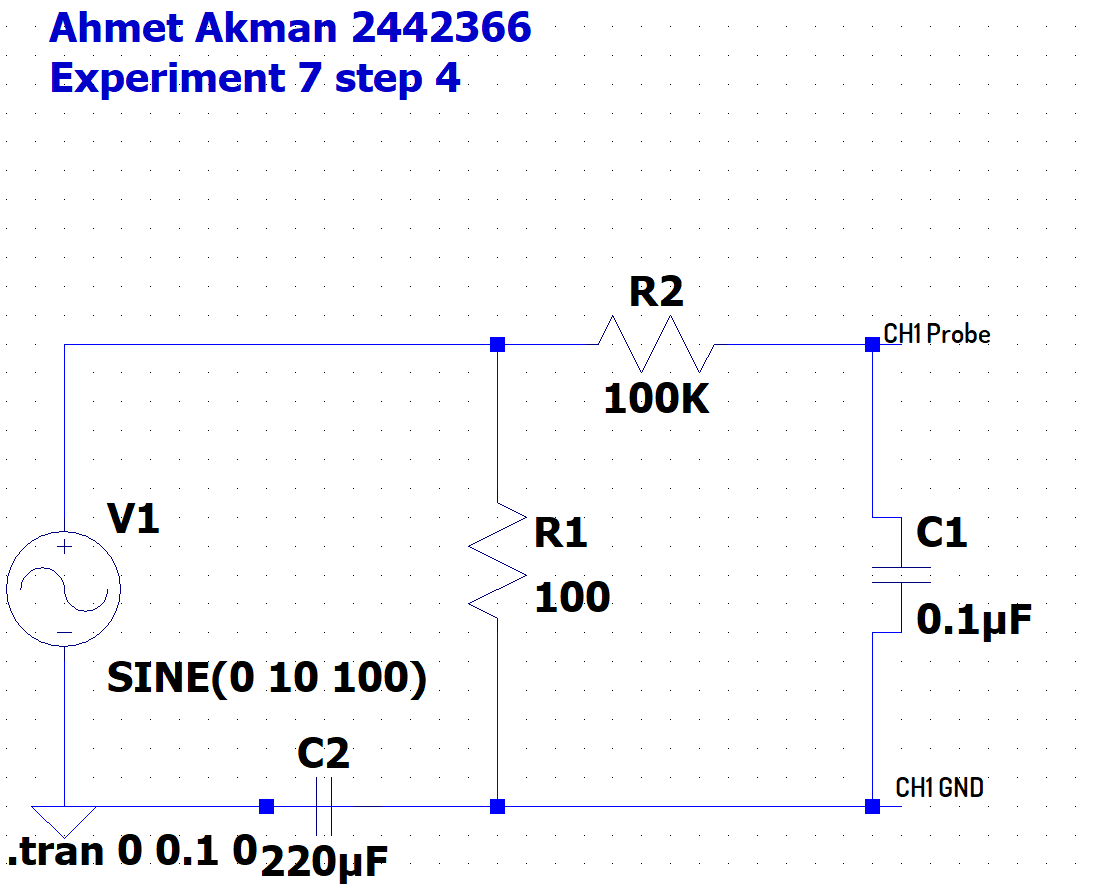
\includegraphics[width=1\textwidth]{4_SCH.png}
   \caption{Simulation circuit for the capacitance finding method}
\end{figure}
Then the q-v characteristics of the capacitor C is plotted as given in Figure 9.
\begin{figure}[H]
	\centering
   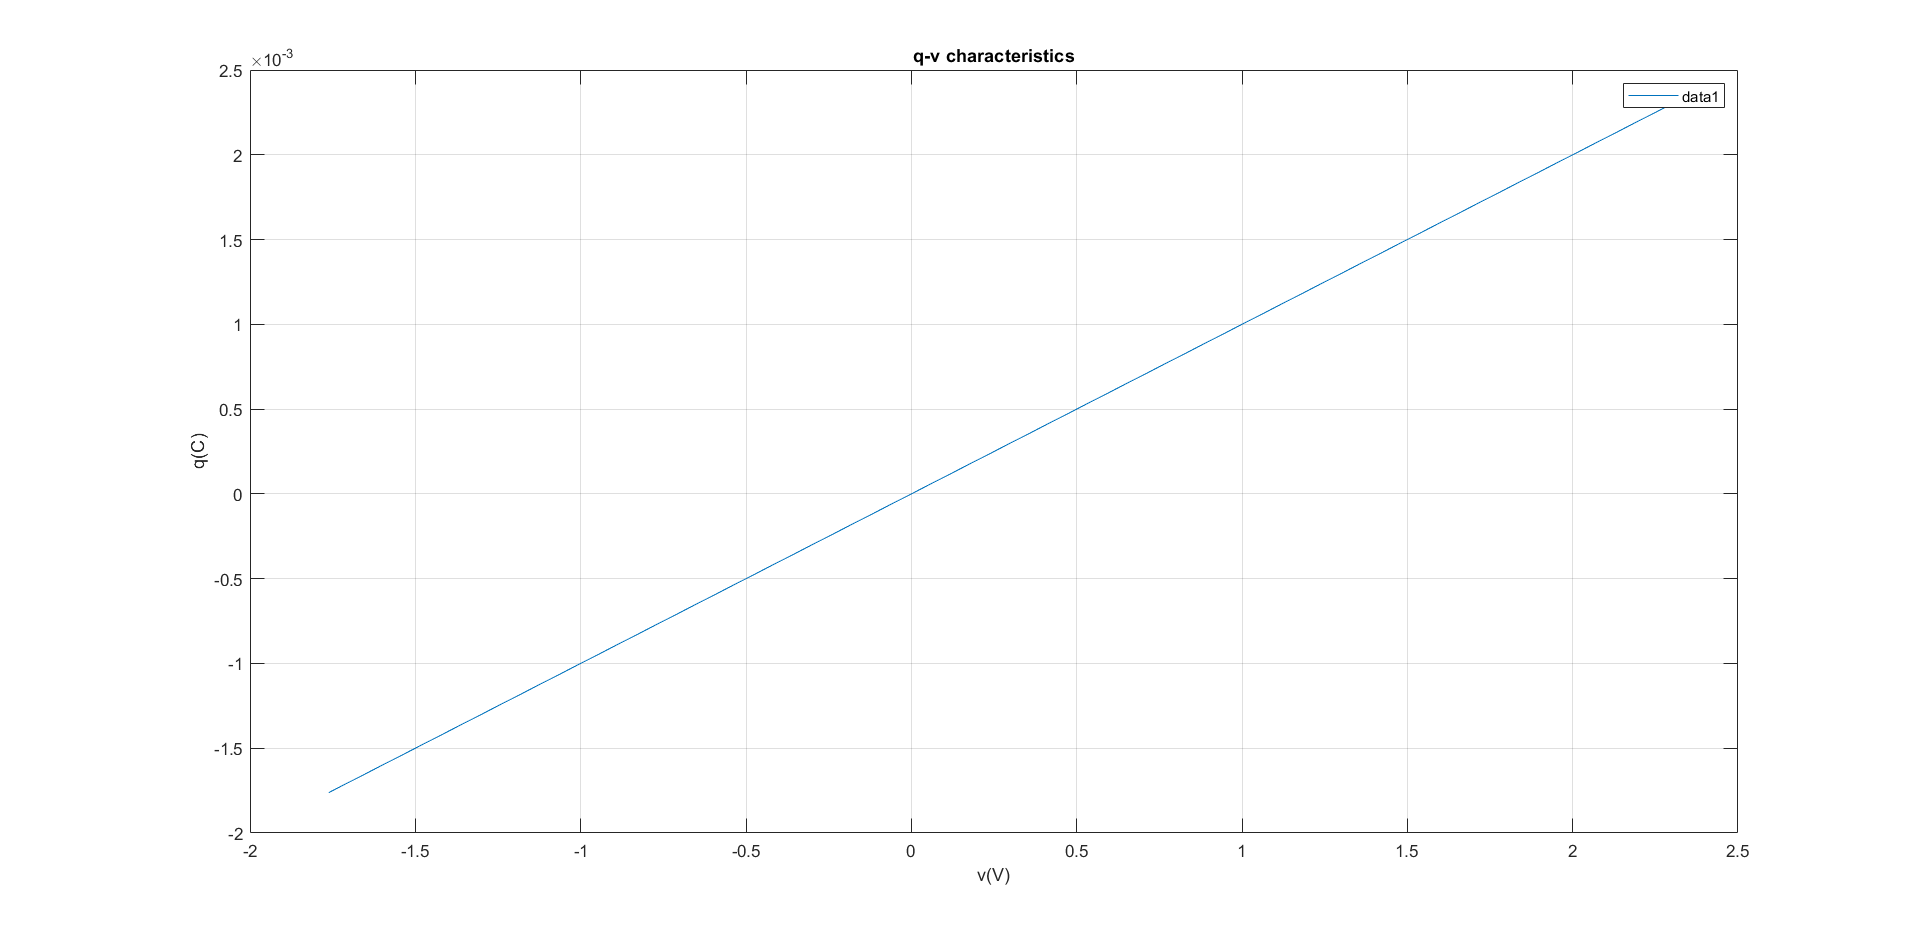
\includegraphics[width=1\textwidth]{4a_plot.png}
   \caption{q-v characteristics}
\end{figure}
The plot is obtained using only \(V_2\) measurement and calculations as follows,
\[ i_2(t) = C_1 \frac{d V_2}{dt} = \frac{V_1(t)}{R_1}
\]
\[
	V_2(t) = \frac{1}{R_i C_i} * \int_{-\infty}^{t} V_1(\tau) \, d\tau
	\]
	\[
		V_2(t) = \frac{R}{R_i C_i} * \int_{-\infty}^{t} i_1(\tau) \, d\tau
		\]
So, 
\[ q(t) = C V_c(t) = \int_{-\infty}^{t} i_1(\tau) \,\tau = \frac{R_i C_i V_2(t)}{R} \]
This mathematical expression helped us to obtain q-v characteristics of the capacitor C on the circuit given in Figure 8.

%%%% MATHEMATICAL RELATION
\subsection{Step 5}
For this step the circuit shown in Figure 6 used ,but the only difference is there used an inductor instead of a capacitor. Firstly, the measurements are made using wooden inductor. The measurements are given in Table 3.
\begin{table}[H]
	\begin{center}
		\caption{Measurements for the wooden inductor circuit}
		\vspace{2mm}
		\begin{tabular}{||c | c | c||} 
		 \hline
		   & Inductor & Resistor \\ [0.5ex] 
		 \hline\hline
		 Voltage Reading & 0.68321 V & 1.862 V \\
		 \hline
		\end{tabular}
\end{center}
\end{table}
Then measurements are conducted for the compact type inductor which is given in Table 4.
\begin{table}[H]
	\begin{center}
		\caption{Measurements for the compact inductor circuit}
		\vspace{2mm}
		\begin{tabular}{||c | c | c||} 
		 \hline
		   & Inductor & Resistor \\ [0.5ex] 
		 \hline\hline
		 Voltage Reading & 0.59929 V & 1.912 V \\
		 \hline

		\end{tabular}
\end{center}
\end{table}
Also the inductance and resistance values are measured for both wooden and the compact inductor. For inductance LC meter is used. Resistance is measured via digital multimeter. The results are given in Table 5.
\begin{table}[H]
	\begin{center}
		\caption{Measurements for the inductors}
		\vspace{2mm}
		\begin{tabular}{||c | c | c||} 
		 \hline
		   & Wooden & Compact \\ [0.5ex] 
		 \hline\hline
		LC Meter Reading & 0.15 H & 0.08 H \\
		 \hline
		Resistance Reading & 29.13 \(\Omega\) & 3.950 \(\Omega\) \\
		 \hline
		\end{tabular}
\end{center}
\end{table}
%%MATHEMATİCAL EXPRESSİON
Therefore the inductance values are calculated using the measurements in Table 7 and the following equation,
\[|Z_c| = \omega L = \frac{V_{RMS}}{i_{RMS}}\]
so,
\[C = \frac{V_{RMS} }{i_{RMS} \omega}
	\]
The results are given in Table 6.
\begin{table}[H]
	\begin{center}
		\caption{Calculation result for the inductors}
		\vspace{2mm}
		\begin{tabular}{||c | c | c||} 
		 \hline
		   & Wooden & Compact \\ [0.5ex] 
		 \hline\hline
		Calculation result & 0.1168 H & 00.0998 H \\
		 \hline
		\end{tabular}
\end{center}
\end{table}
The results shows that, our approximations are quite consistent with the real world value. The deviation is stemmed from the neglected resistance of the inductors which are given in Table 5. By adding them to the equation , the calculation can be resulted more accurately.
\subsection{Step 6}
Circuit given in Figure 10 is set for this step. The variables set as \(V_{in}\) = 10sin(2*\(\pi\) ft) V , f = 5kHz and \(L_1\) = H.
\begin{figure}[H]
	\centering
   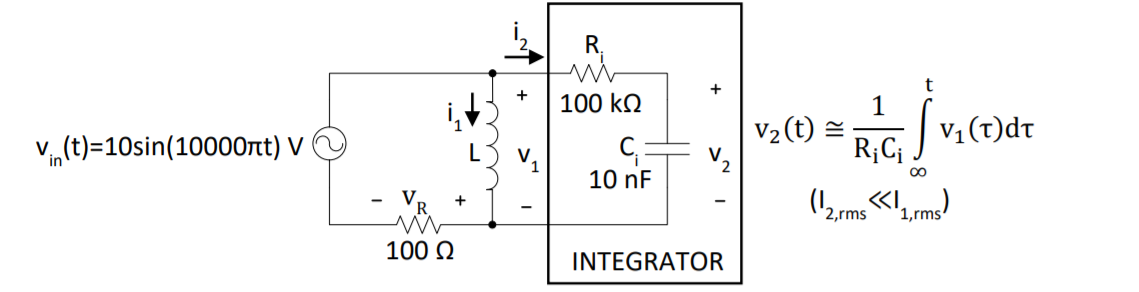
\includegraphics[width=1\textwidth]{PRE7.png}
   \caption{Circuit for the inductance finding method}
\end{figure}

\subsubsection{a)}
The circuit schematic given in Figure 11 is constructed in LTSPice simulation environment.
\begin{figure}[H]
	\centering
   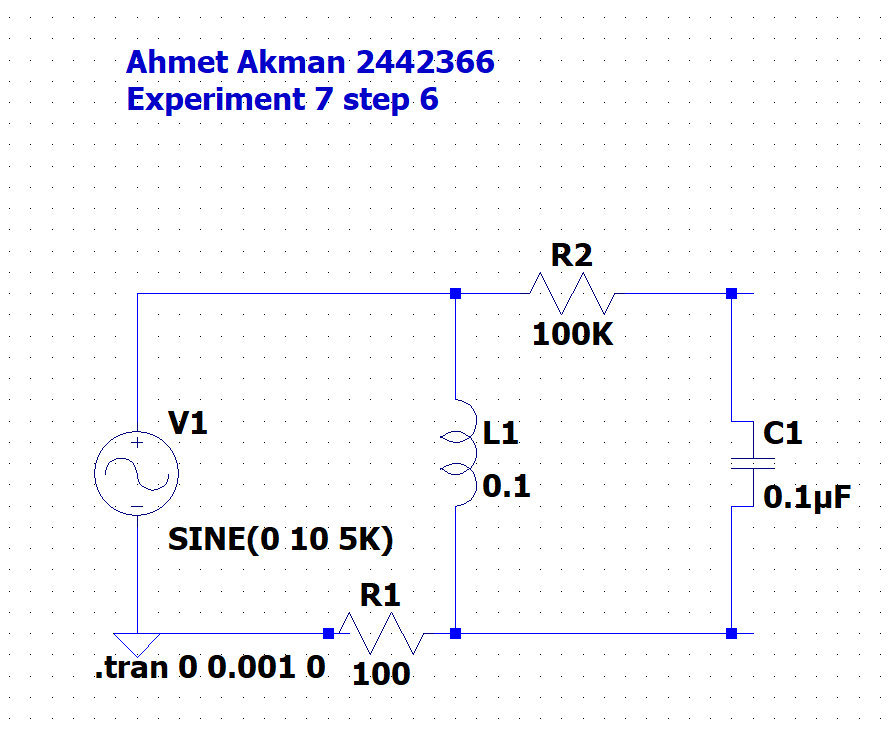
\includegraphics[width=1\textwidth]{6_SCH.png}
   \caption{Simulation circuit for the inductance finding method}
\end{figure}
Then using the following relation obtained in the Preliminary work the plot shown in Figure 12 is obtained.
\[
i_1*100 = V_R
\]
\[
	\phi(t) = L i(t) = \frac{L V_R}{100}
\]
by the equation given in Figure 10,
\[V_2 R_i C_i = L i(t)\]
\[V_2 R_i C_i = \frac{L V_R}{100}\]
\[L = \frac{100 V_2 R_i C_i}{V_R}\]
also,
\[\phi(t) = V_2 R_i C_i\]

\begin{figure}[H]
	\centering
   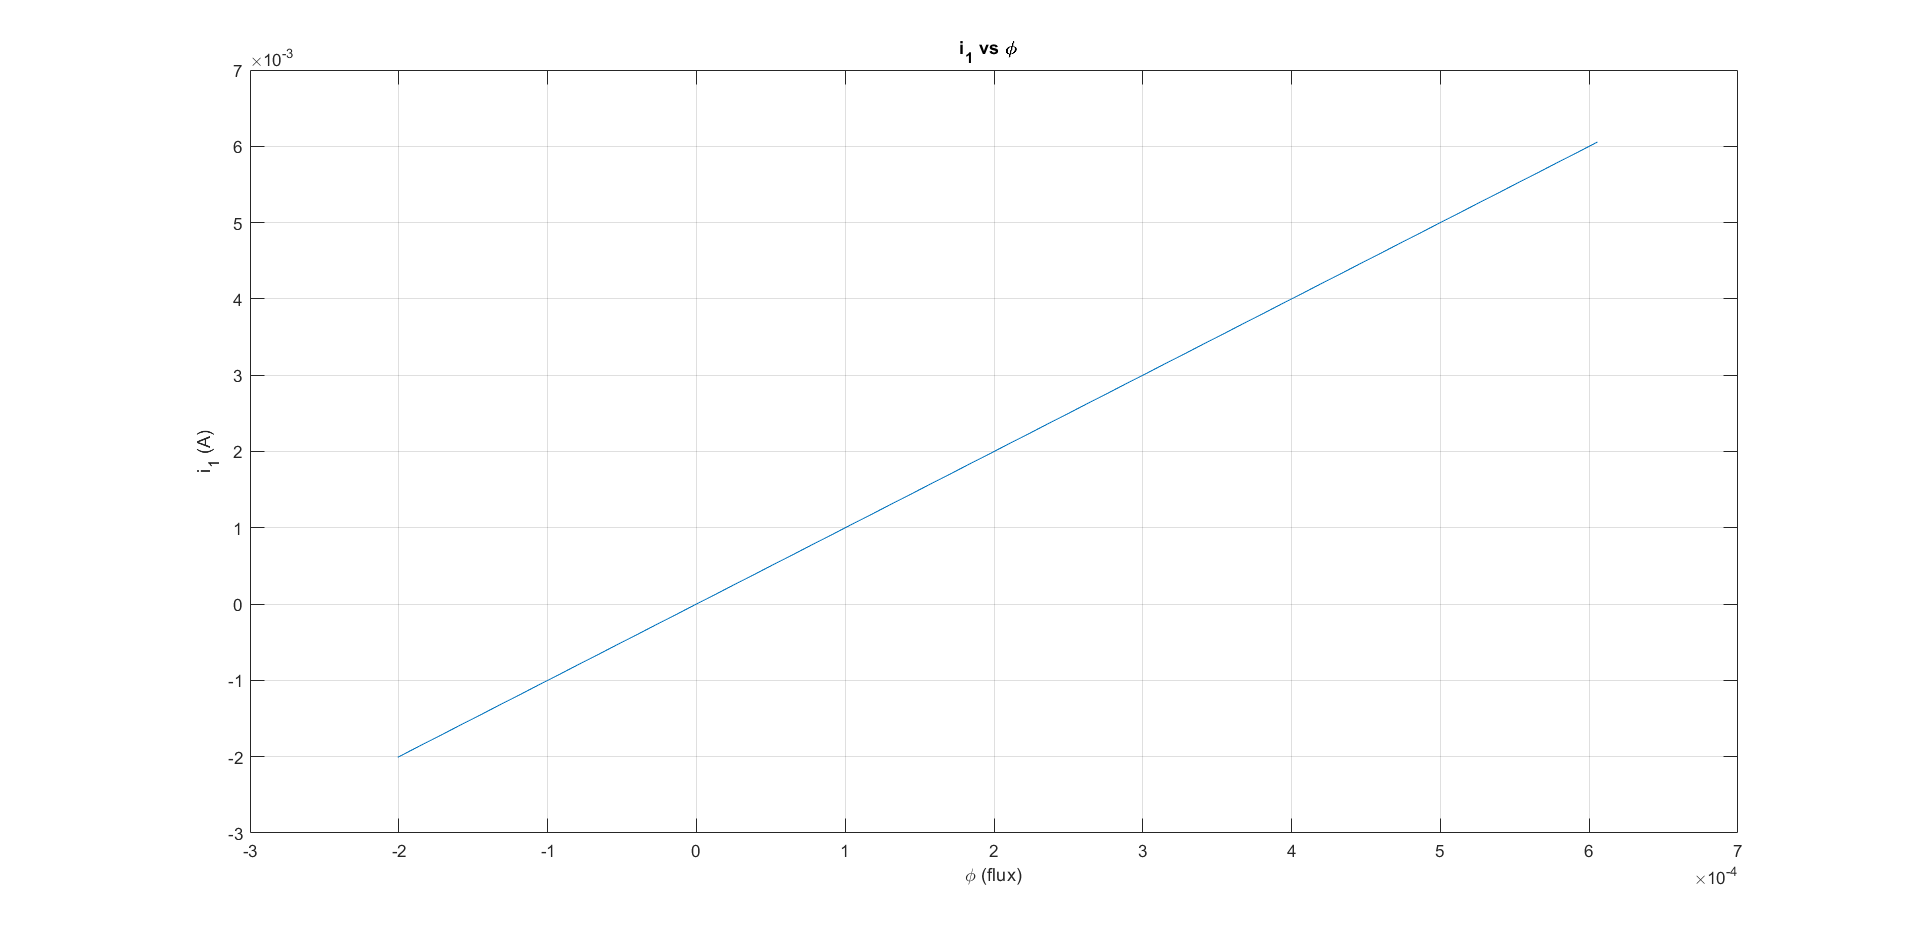
\includegraphics[width=1\textwidth]{PRE_7c.png}
   \caption{\(\phi vs i\) characteristics plot}
\end{figure}
It can be seen that there is a linear relation between flux and current on an inductor.
\subsubsection{b)}
In the lab video, Advance Signal Generator used for this step. This is stemmed from the fact that Agilent signal generator is not able to provide floating signal, it only can supply grounded signal. So since Advance Signal Generator which operates analog, is able to supply floating signal it is used. 
\section{Conclusion}
The non-ideal behavior of the components is compared with the ideal simulation plots.

In conclusion, in experiment 7, "Rectifiers, Capacitors and Inductors," as students, we have learned how various functional circuit setups rectifiers constructed. Preliminary laboratory work is done via simulations of rectifier, capacitor and inductor circuits in an LTSpice environment and by mathemaical relations. As students, we have seen how half wave and full wave rectifiers behave. We have inferred the capacitance and inductance values indirectly and compared with the direct ones. The characteristics of the q-v and \(\phi\)-i are observed with the help of their calculations. Lastly, different inductors and their behaviors are observed ,and the mathemaical expressions verified via measurements. To sum up, in this experiment, as students, we have experimented with how different rectifier circuit operate, how can we measure or calculate the inductance and capacitance values. 
\section*{Appendix I}
Total time spent on/during:
\begin{itemize}
	\item Pre-lab preparation: 4.5 hours (including the preliminary work and simulations) 
	\item Experimental work: 2 hours (hours spent in lab)
	\item Report writing: 3 hours 
\end{itemize}
\section*{Appendix II}
The outputs of the simulations are fetched from LTSpice and plotted in MATLAB. 
%++++++++++++++++++++++++++++++++++++++++
% References section will be created automatically 
% with inclusion of "thebibliography" environment
% as it shown below. See text starting with line
% \begin{thebibliography}{99}
% Note: with this approach it is YOUR responsibility to put them in order
% of appearance.

%\begin{thebibliography}{99}

%https://tr.overleaf.com/latex/templates/sample-lab-report-for-u-of-r-phys-349/pgsyqngcyjxk

%\end{thebibliography}


\end{document}


\begin{table}[H]
	\begin{center}
		\caption{Resistance reading by color code convention.}
		\vspace{2mm}
		\begin{tabular}{||c | c | c||} 
		 \hline
		 Color Order & Value & Tolerance \\ [0.5ex] 
		 \hline\hline
		 Brown / Black / Red / Gold & 1k\( \Omega \) & \( \% \) 5  \\ 
		 \hline
		 Yellow / Violet / Red / Gold & 4.7k\( \Omega \) & \( \% \) 5   \\
		 \hline
		 Brown / Grey / Orange / Gold & 18k\( \Omega \) & \( \% \) 5  \\ [1ex] 
		 \hline
		\end{tabular}
	\end{center}
	\end{table}

	\begin{figure}[H]
 		\centering
		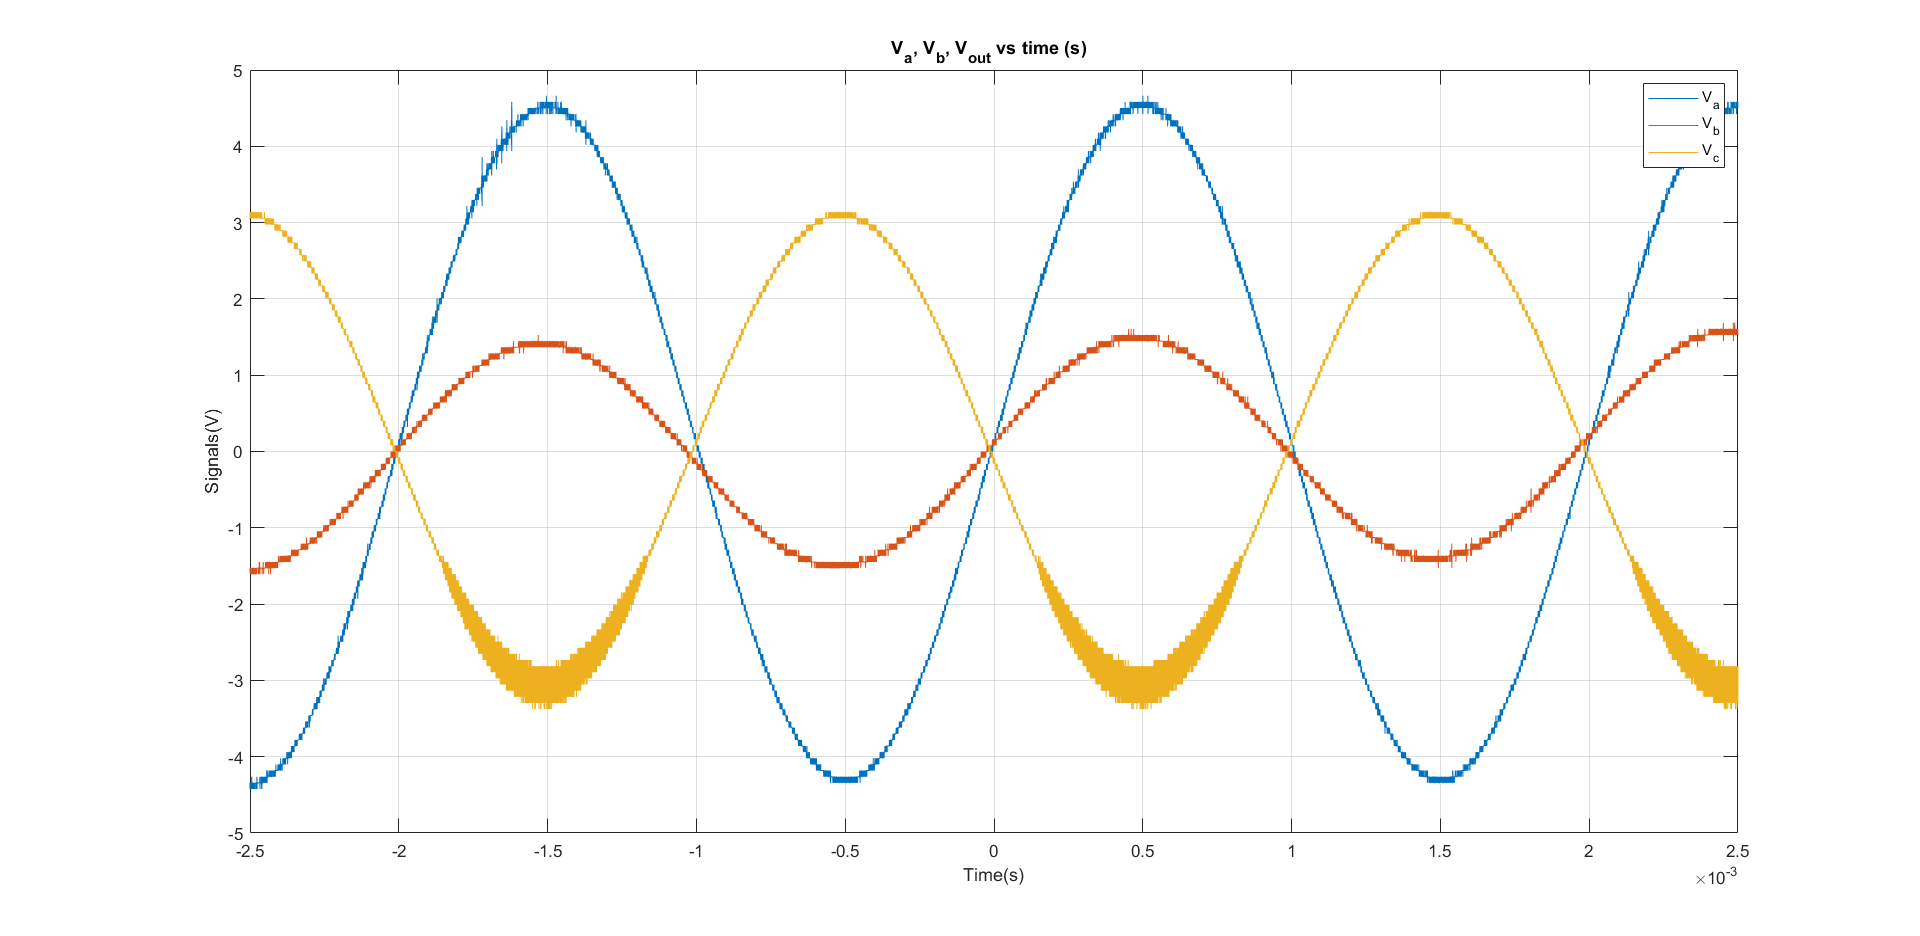
\includegraphics[width=0.6\textwidth]{5.png}
		\caption{Circuit schematic for the step 5}
	\end{figure} 

	\begin{figure}[htp] \centering{
		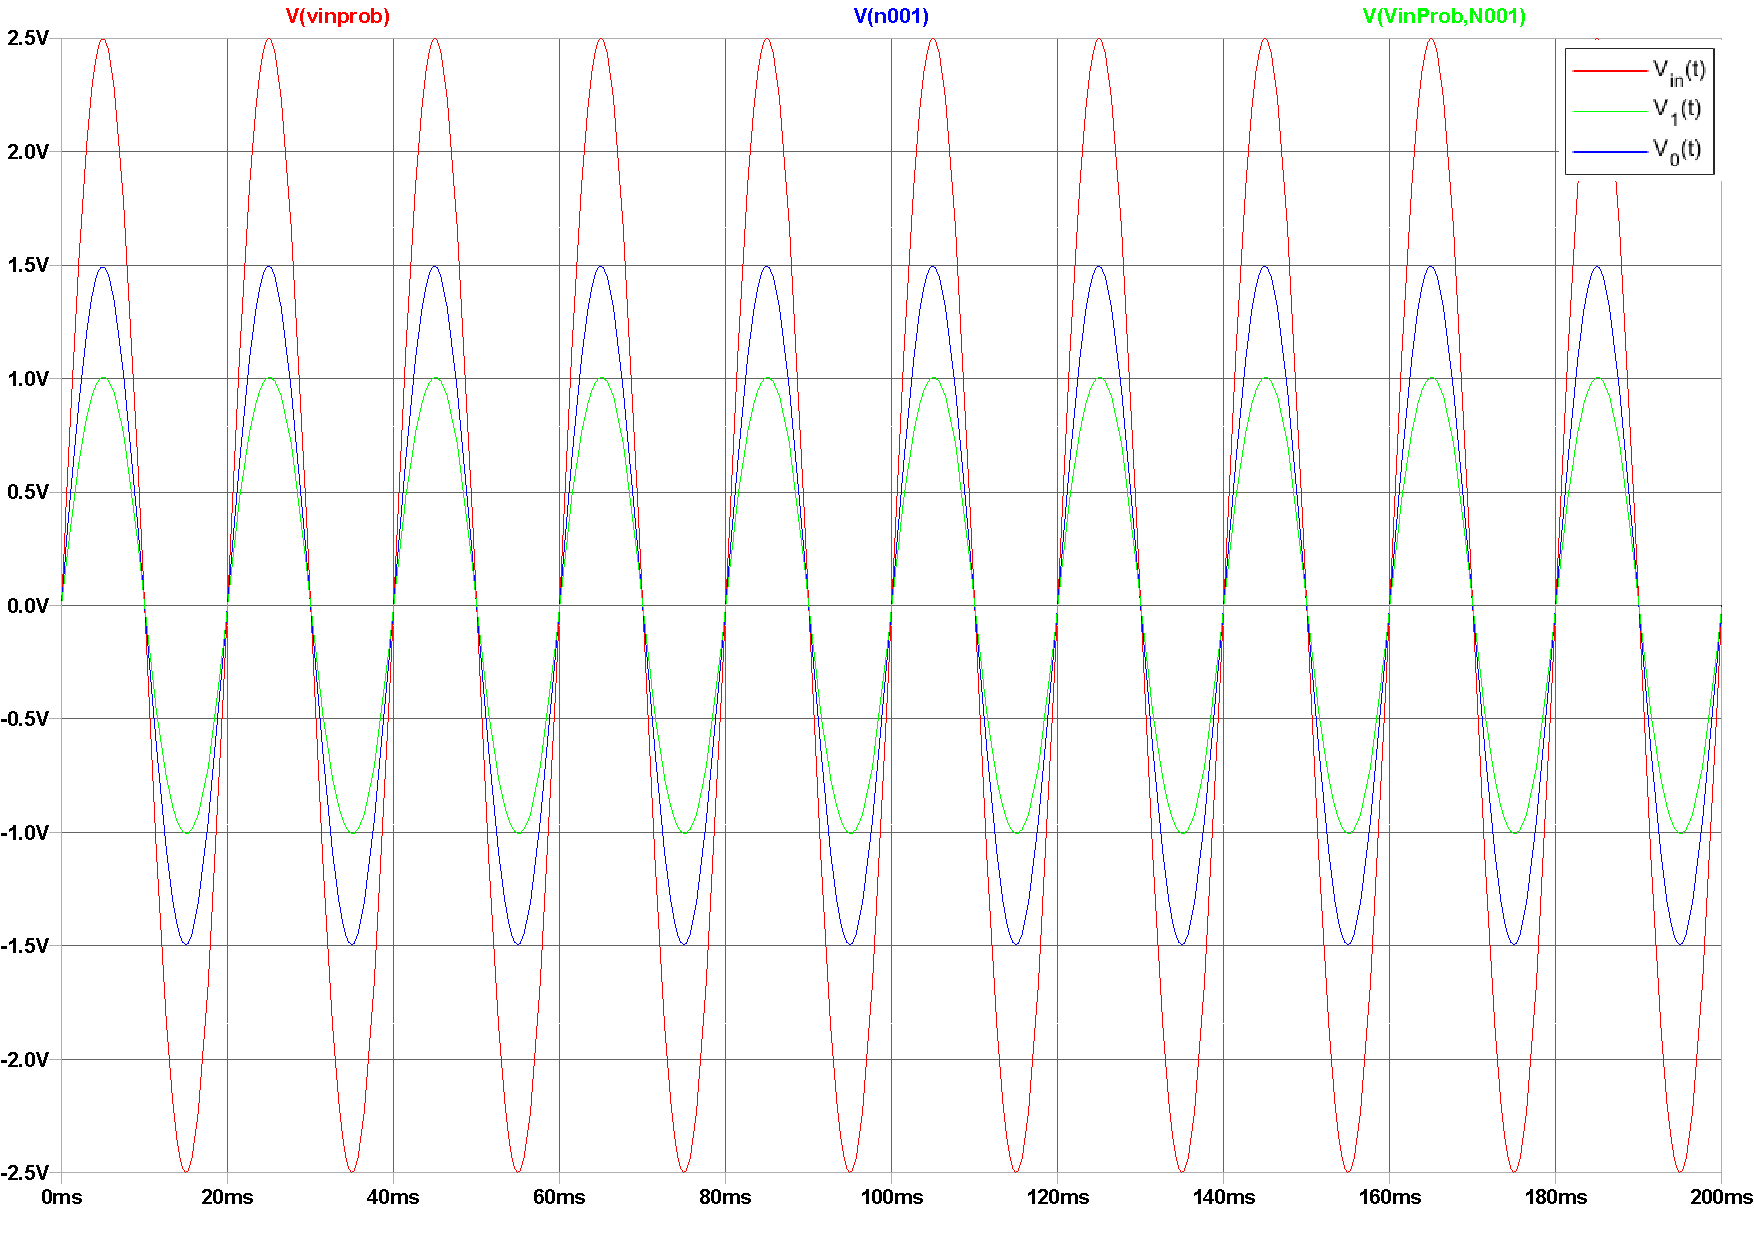
\includegraphics[scale=0.25]{2a_plot.pdf}}
		\caption{Experiment 2}
\end{figure}
	